% Literature review for the first meeting

\documentclass[a4paper,11pt,twoside]{article}
\usepackage[T1]{fontenc}
\usepackage[utf8]{inputenc}
\usepackage{color,dcolumn,graphicx,hyperref}
\usepackage{wrapfig}
\usepackage[top=2.5cm, bottom=2.5cm, left=2.5cm, right=2.5cm]{geometry}
\usepackage{setspace}
\onehalfspacing
\usepackage{scrextend}
\addtokomafont{labelinglabel}{\sffamily}
\usepackage[round]{natbib}
\bibliographystyle{abbrvnat}
\usepackage{tcolorbox}
\usepackage{filecontents}
\usepackage{csquotes}
\usepackage{epigraph}
\usepackage{ragged2e}
\usepackage{wrapfig}
\usepackage[font=small]{caption}
\hypersetup{
  colorlinks = true,
  allcolors=[rgb]{0,0.4,0.5},
}

%% Packages for Graphics & Figures
\usepackage{graphicx} %%For loading graphic files
\usepackage{float}

%% Math Packages
\usepackage{amsmath}
\usepackage{amsthm}
\usepackage{amsfonts}


\begin{document}

\title{Linking forest management and species distribution models: a theoretical approach under climate change}

\author{Willian Vieira}

\maketitle

\begin{abstract}

Abstract section

\end{abstract}

\begin{displayquote}
\centering\textit{Ecology may provide many of the answers — but only if it is holistic enough to incorporate the human element as part and parcel of the ecosystem.} \\ \RaggedLeft{\citep[p. 231]{Pfister1993}}
\end{displayquote}

\section{What is going on?}

\textit{I can use the section in the Robert's project}\\
Climate change is an increasing trending topic both in non-scientific \citep{Capstick2015} and scientific environment (Figure \ref{fig:fig1}), transforming our world as a metamorphosis of practice and acting \citep{Beck2016}.
According to IPCC \citep{Cubasch2013}, humans activities are contributing to increase the concentration of greenhouse gases, which can lead to increase the mean temperature and the strength of extreme climate events.
This global change has an impact in different biological processes, from local species constraints \citep[e.g. low regeneration][]{Treyger2011} to shift in species' range \citep{Boisvert-Marsh2014,Monleon2015} and in community composition \citep{Dieleman2015}, impacting biodiversity at different scales \citep{Penuelas2013}.

\begin{wrapfigure}{r}{0.38\textwidth}
    \centering
    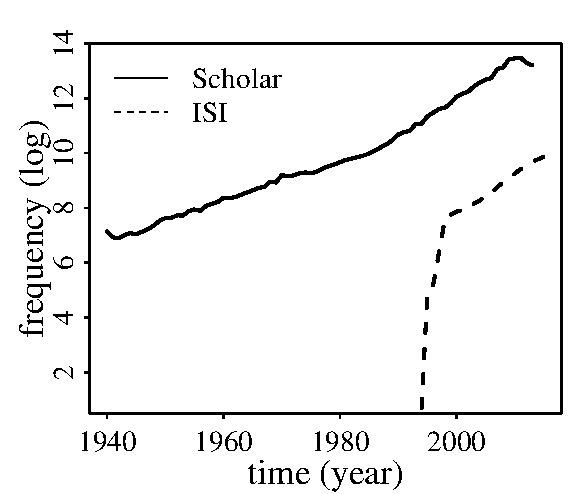
\includegraphics[width=0.38\textwidth]{img/fig1_em.pdf}
    \caption{Frequency of the keyword ``Climate change'' used in research papers indexed on Google Scholar (1940 - 2013) and Web of Science (1994 - 2015)}
    \label{fig:fig1}
\end{wrapfigure}

Species distribution models (SDM; defined in section \ref{sdm}) has predicted tree species' range shift under climate change, providing a wide range of applications, as in biodiversity conservation and management \citep{Guisan2005,Guisan2013}.
However, these models are generally phenomenological and  distributed at equilibrium with climate \citep[e.g.][]{Pigot2013}.
Hence, they do not consider important determinants of range limits as demography \citep{Louthan2015}, biotic constraints \citep{Wisz2013,Pigot2013} and species absences data \citep{Koshkina2017}, inducing non-accurately projection of the future spatial distribution of a species.
Considering then ecological constraints, trees' migration rate following climate change will be slower than predicted \citep{Bertrand2011,Sittaro2017}, increasing the climatic debt \citep{Bertrand2016}.

%climate debt and extinction debt are similar?
The climatic debt is a measure of the lag (or disequilibrium) of plant communities with climate change, integrated in an environmental context \citep{Bertrand2016}.
\citet{Essl2015} has listed twelve mechanisms that contribute to delayed biodiversity responses, among them, changes appears at ecosystem (loss and degradation), community (secessional, biotic interaction, species removal and invasion) and population (evolutionary and adaptive) levels.
Disturbance regime was also listed but it may not by related to climate debt \citep{Bertrand2016}.
Hence, this lag under climate change promotes extinction debt, being a challenging for biodiversity conservation \citep{Kuussaari2009} and productivity \citep{Lasch2002}.
Then identify the mechanisms shaping delayed biotic response to environment is crucial to access the vulnerability of biodiversity to climate change and improve forecasts and biodiversity management \citep{Essl2015,Bertrand2016}.
%find a way to add forest management here. Have to create a link to the next section. 

\section{What should we do?}

Increase forest resilience! \textbf{(i)} But what is it exactly? (paper: Building evolutionary resilience for conserving biodiversity under climate change) Try and discuss this aspect in different perspectives. \textbf{(ii)} Why resilience?

\textbf{Forest management}

Present some motivations, advantages and disadvantages in considering forest management.

Interesting argument about who should peak do winners from \citet{Webster2017}. They say that \textit{Predict-and-prescribe management may erode diversity by focusing on ‘winners’}.

Forest management in a theoretical view was actually not very much explored and so I consider it a kind of gap we should better explore. Read \citet{Becknell2015} for an overview.

\section{Study case: the Quebec forest resource}

Explain here where I am going to work and also why I am choosing this area.

\section{Theoretical approach}

Read the section \textit{recent developments in predicting changes in species distribution} from \citet{Ehrlen2015}

\subsection*{Disturbance}
Pass through the main disturbance theories basing mainly in \citet{Pulsford2016} (verify with Dom if this section is necessary)

\subsection*{Resilience}
\textbf{(iii)} But how to calculate it in a analytical way? Before introduce the method to calculate resilience, we must have an idea of what is the equilibrium (\hyperlink{box1}{Box 1}) and stability (\hyperlink{box2}{Box 2}) of a model. Now introduce the calculus of $\lambda$ by Jacobian matrix.

\begin{tcolorbox}
\hypertarget{box1}{Box 1}. Equilibrium
\begin{align}
E &= mc^2 & \text{Formula of the universe}
\end{align}
\end{tcolorbox}

\begin{tcolorbox}
\hypertarget{box2}{Box 2}. Stability
\begin{align}
E &= mc^2 & \text{Formula of the universe}
\end{align}
\end{tcolorbox}

\subsection*{Range dynamics theory}

What theories can help us to describe species range under climate change?\\
How to integrate forest management in this theory?\\
-> Matapopulation dynamics theory <-

\subsection*{Transition period}


\subsection*{Species Interaction: why is it important?}
Explain the role species interaction can play on its distribution range.
http://www.sciencedirect.com/science/article/pii/S0169534715002475
The perceived threat of climate change is often evaluated from species distribution models that are fitted to many species independently and then added together. This approach ignores the fact that species are jointly distributed and limit one another \citep{clark2014}.

Joint species distribution?

Interactions between land-use and climate also can underestimate species resilience in distribution models \citep{Goring2017}.

\section{How to do it?}

Here we see a briefly presentation of possible methods will be used in the thesis.

\subsection*{Modeling}

Why and how modeling?\\
Morin et thuiller 2009:{What then are the best strategies for obtaining accurate predictions for changes in the distributions of deciduous temperate trees? At the scale of the geographic distribution of species, no experiments in situ can be reasonably carried out to predict possible range shifts (Woodward 1987). Modeling therefore appears the most feasible and efficient way to establish useful predictions (Lovejoy and Hannah 2005, Thuiller 2007), and several kinds of models have been developed during the previous decade for this purpose. As reviewed by Midgley et al. (2007), these models fall into two main classes: vegetation-type models (dynamic global vegetation models [DGVMs]) and species-specific models (niche-based and process-based).}

\subsubsection*{Species Distribution Models}\label{sdm}

Nice resume about SDM in \citet{Moran-Ordonez2016}.

\subsubsection*{Integral Projection Models}

\textit{I should be writing and not playing with \LaTeX}

\subsection*{Bayesian approach}

\textit{I should be writing and not playing with \LaTeX}

\section{Thesis structure}

The first part of the thesis will be a general introduction in French where  I will probably use a part of this document and present the big picutre of my thesis.

The first chapter will try to answer the question \textit{Can forest management increase forest resilience to climate change?}. The paper will work with an analytical and sensitivity analysis in a metapopulation dynamics model to understand the impact of forest management on increasing forest resilience.

In the second chapter I am going to build a landscape model that will consider both forest management and species interaction.

The third chapter I am going to build another model but in a local scale. \textit{I have to find a good biological reason for that}.

The fourth chapter will then integrate both landscape and local model into one. Here I will also track the uncertainty of the model by bayesian approach.


TODO: \\
- Automate box labels \\
- Short reference style \\

\bibliography{/users/wvieira/Documents/mendeley_bibtex/Thesis.bib}

\end{document}
